\documentclass[tikz,border=2mm]{standalone}
\usepackage[T1]{fontenc}
\usepackage[utf8]{inputenc}
\usepackage[scaled]{helvet}
\renewcommand{\familydefault}{\sfdefault}
\usetikzlibrary{arrows.meta,positioning,calc}
\definecolor{dunkel}{HTML}{1F3A5F}
\definecolor{mittel}{HTML}{5B7FA6}
\definecolor{hell}{HTML}{DCE6F0}
\definecolor{text}{HTML}{222222}
\tikzset{
  every node/.style={text=text},
  pfeil/.style={line width=2pt,draw=dunkel,-{Triangle[length=3.5mm,width=4mm]}},
  doppelpfeil/.style={line width=4pt,draw=dunkel,{Triangle[length=4mm,width=7mm]}-{Triangle[length=4mm,width=7mm]}},
  duennpfeil/.style={line width=1pt,draw=mittel,{Stealth[length=2.5mm]}-{Stealth[length=2.5mm]}},
}

\usepackage{fontawesome5}
\begin{document}
\begin{tikzpicture}[
    font=\footnotesize,
    every node/.append style={execute at begin node={\hyphenpenalty=10000\exhyphenpenalty=10000}},
    schritt/.style={fill=#1,rounded corners=1.5mm,minimum width=2.4cm,minimum height=1.05cm,
      align=center,text width=2.2cm,text=grund,font=\footnotesize\bfseries},
    schritt/.default=dunkel,
    info/.style={draw=schrift,fill=grund,rounded corners=2mm,align=center,text width=2.3cm,
      inner sep=1.2mm,font=\scriptsize},
    symbol/.style={circle,draw=schrift,fill=grund,line width=0.6pt,inner sep=0.6mm,
      minimum size=6.5mm,font=\small},
    linie/.style={line width=0.6pt,draw=schrift},
    fluss/.style={line width=0.8pt,draw=schrift,-{Triangle[length=2mm,width=2mm]}},
  ]
  % Magnifier with the final draft; the lens covers the start of the zoom lines
  \draw[line width=1pt,draw=hell] (1.2,4.1) -- (3.05,8.6);
  \draw[line width=1pt,draw=hell] (1.2,4.1) -- (3.05,-0.6);
  \draw[line width=2.2mm,draw=schrift,line cap=round] (1.75,3.25) -- (2.6,2.4);
  \filldraw[draw=schrift,line width=2mm,fill=hell] (1.2,4.1) circle (1.05);
  \node[draw=schrift,fill=grund,minimum width=1.1cm,minimum height=1.45cm,align=center,
    font=\small\bfseries] at (1.2,4.1) {Final\\draft};

  % Main path
  \node[schritt] (ao) at (4.4,4.1) {Advanced organizer};
  \node[schritt] (ctx) at (7.2,4.1) {1. Context};
  \node[schritt=akzent] (s2) at (10.3,6.1) {2. Alignment with chemistry class};
  \node[schritt=akzent] (s3) at (13.2,6.1) {3. Inquiry methods};
  \node[schritt=mittel] (i2) at (10.3,2.1) {2. Alignment with chemical industry};
  \node[schritt=mittel] (i3) at (13.2,2.1) {3. Inquiry methods};
  \node[schritt] (prep) at (16.3,4.1) {4. Preparation tasks};
  \node[schritt] (flow) at (19.2,4.1) {Flowchart};
  \node[draw=schrift,fill=grund,line width=0.6pt,minimum width=1.9cm,minimum height=1.6cm,
    align=center,font=\footnotesize\bfseries,text width=1.7cm] (manual) at (21.9,4.1)
    {Traditional laboratory manual};
  \fill[grund] ([xshift=-3mm]manual.north east) -- (manual.north east) -- ([yshift=-3mm]manual.north east) -- cycle;
  \draw[line width=0.6pt,draw=schrift] ([xshift=-3mm]manual.north east) -- ([xshift=-3mm,yshift=-3mm]manual.north east) -- ([yshift=-3mm]manual.north east);

  \draw[fluss] (ao) -- (ctx);
  \draw[linie] (ctx.east) -- (8.6,4.1);
  \draw[fluss] (8.6,4.1) |- (s2.west);
  \draw[fluss] (8.6,4.1) |- (i2.west);
  \draw[fluss] (s2) -- (s3);
  \draw[fluss] (i2) -- (i3);
  \draw[linie] (s3.east) -| (14.8,4.1);
  \draw[linie] (i3.east) -| (14.8,4.1);
  \draw[fluss] (14.8,4.1) -- (prep.west);
  \draw[fluss] (prep) -- (flow);
  \draw[fluss,dashed] (flow) -- (manual);

  % Symbols on the boxes
  \node[symbol,anchor=south] at (ctx.north) {\faBatteryFull};
  \node[symbol,anchor=north] at (s2.south) {\faChalkboardTeacher};
  \node[symbol,anchor=north] at (s3.south) {\faFlask};
  \node[symbol,anchor=south] at (i2.north) {\faIndustry};
  \node[symbol,anchor=south] at (i3.north) {\faFlask};
  \node[symbol,anchor=south] at (prep.north) {\faClipboardList};

  % Descriptions
  \node[info] (ao1) at (4.4,2.6) {Overview of the content of the material};
  \node[info] (ctx1) at (7.2,2.6) {Brief theoretical background and visualization};
  \node[info,inner sep=0.8mm] (ctx2) at (7.2,0.8) {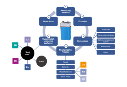
\includegraphics[width=2.2cm]{bitmaps/context_visualisierung.png}};
  \node[info] (s2a) at (10.3,7.65) {Taking the role of a teacher};
  \node[info] (s2b) at (10.3,8.75) {Possible application of the context in school};
  \node[info] (s3a) at (13.2,7.65) {Relevance for teachers};
  \node[info] (s3b) at (13.2,8.75) {Which important inquiry methods are taught in the analysis?};
  \node[info] (i2a) at (10.3,0.55) {Taking the role of an employee};
  \node[info] (i2b) at (10.3,-0.6) {Connection between context and the inquiry methods needed in chemical industry};
  \node[info] (i3a) at (13.2,0.55) {Relevance for chemical industry};
  \node[info] (i3b) at (13.2,-0.6) {Which important inquiry methods are taught in the analysis?};
  \node[info] (prep1) at (16.3,2.5) {Reflection of the inquiry methods for the analysis in the lab};
  \node[info] (flow1) at (19.2,2.3) {Visual connection between contextualized pre-lab materials and traditional analysis in the lab};
  \node[info,inner sep=0.8mm] (flow2) at (19.2,7.3) {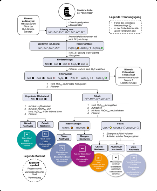
\includegraphics[width=2.2cm]{bitmaps/context_flowchart.png}};

  \draw[linie] (ao) -- (ao1);
  \draw[linie] (ctx) -- (ctx1);
  \draw[linie] (ctx1) -- (ctx2);
  \draw[linie] (s2) -- (s2a);
  \draw[linie] (s2a) -- (s2b);
  \draw[linie] (s3) -- (s3a);
  \draw[linie] (s3a) -- (s3b);
  \draw[linie] (i2) -- (i2a);
  \draw[linie] (i2a) -- (i2b);
  \draw[linie] (i3) -- (i3a);
  \draw[linie] (i3a) -- (i3b);
  \draw[linie] (prep) -- (prep1);
  \draw[linie] (flow) -- (flow1);
  \draw[linie] (flow) -- (flow2);
\end{tikzpicture}
\end{document}
